\section{Definition von SIEMs und Log-Analyse-Tools}

Sowohl in der wissenschaftlichen als auch in der kommerziellen Literatur gibt es verschiedene Definitionen von \gls{SIEM}. Diese widersprechen sich nicht, aber zeigen unterschiedliche Perspektiven. Eine von dieser Definitionen behaupt, dass \gls{SIEM} das Ergebnis einer Kombination zwischen dem \glsfirst{SEM} und \glsfirst{SIM} ist \citep{Dorigo_SIEM}. Das Erste bezieht sich auf die Identifizierung, Bewertung, Beobachtung und den Bericht von Sicherheitsvorfällen mithilfe von verschiedenen Log Dateien \citep{techopedia_SEM}. Das Zweite ist eine Software, die bei der automatischen Sammlung von Loginformationen aus vielen Quellen, wie Firewall und Servern unterstützt \citep{techopedia_SIM}. Da die meisten \gls{SIEM}-Lösungen kostenpflichtig sind, existieren auch viele \gls{opensource} Log-Analyse-Tools, die eine ähnliche Aufgabe erledigen, ohne die Kernelemente von \gls{SIEM} zu besitzen. 

Log-Analyse-Tools sind in der Regel Anwendungen die Logdateien empfangen, speichern, bearbeiten und nach spezifisichen  Regeln bewerten. Diese Tools unterstützen Programmierer und Systemadministratoren bei der Überwachung des Zustands von Systems oder einer Software. Ein solches Tools kann Logdateien von verschiedenen \glsplural{Endpoint} und in verschiedenen Formaten bekommen, so dass es schließlich einen Bericht oder eine Grafik erzeugt \citep{Korzeniowski_LATDef}. Die Nutzung dieser Tools beschränkt sich nicht auf den Sicherheitsbereich ein, sondern kann für gesamte IT-Bereich  nützlich sein.

In dem Universum des \gls{SOC} mischen sich verschiedene Begriffe, die manchmal zur Verwirrung führen, weil sie ähnliche Bedeutungen haben und Verantwortungen abdecken. \glsfirst{IDS}, \glsfirst{IPS}, \glsfirst{SIEM} und Log-Analyse-Tools werden von Laien und sogar von Spezialisten oft verwechselt, da ihre Aufgaben mehr Gemeinsamkeiten als Unterschiede haben. Diese Tools sind feste Bestandteil eines \gls{SOC}, jedoch konzentrieren wir uns auf Log-Analyse. Um den Fokus der Arbeit zu vergrenzen, erläutern wir im folgenden Abschnitt die erwähnten Begriffe.

\newpage
\glsfirst{IDS}, \glsfirst{IPS} und \glsfirst{SIEM} sind Sicherheitstool als Software und/oder Hardware, die zusammenarbeiten können, um einen umfangreiche Netzwerksicherheit anzubieten. \gls{IDS} identifizieren und berichten über \glsplural{Cyberangriff}, indem er Netzwerkverkehr überwacht. Nach der Erkennung eines verdächtigen Verkehrs, muss das \gls{SOC} Team zur Handlung kommen. \gls{IPS} überwacht den Netzwerkverkehr und kann die Verbindung automatisch unterbrechen, falls es verdächtig ist \citep{Wendzel_IS}. Ein \gls{IPS} kann konfiguriert werden, um automatisch nach festgelegten Muster zu handeln. Beide Tools können Logdateien generieren, die von einer \gls{SIEM}-Lösung oder Log-Analyse-Tools gesammelt werden können. Die folgende Abbildung, \ref{fig:SIEM_Allg_Struktur}, stellt eine allgemeine Struktur von \gls{SIEM}-Lösungen dar:

\begin{figure}[H]
   \centering
   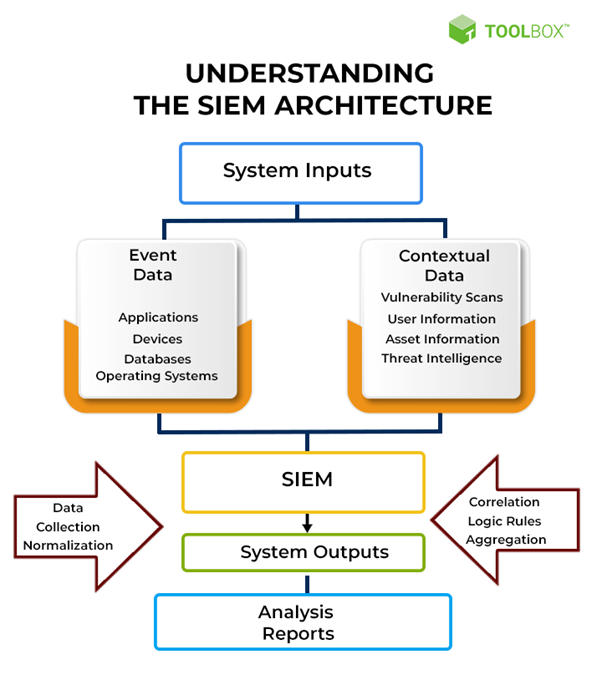
\includegraphics[width=0.55\textwidth]{assets/2_p1.png}
   \caption[Allgemeine Struktur von \gls{SIEM}]
   {Allgemeine Struktur eines \gls{SIEM}\\Quelle: \citep{Mohanan_What} }
   \label{fig:SIEM_Allg_Struktur}
   \centering
\end{figure}

Obem auf dem Bild, sehen wir, dass es zwei wichtige Datenquelle gibt, auf der linken Seite sind die Logdateien der \glsplural{Endpoint} und auf der rechten Seite die Informationen, um Anomalie zu erkennen. Nur der linken Seite stellt ein Log-Analyse-Tool dar. Mit der Nutzung der Elementen der rechten Seite, werden die Daten verarbeitet, um Muster zu erkennen und Information herauszuholen. Diese Zusammenarbeit repräsentiert eine \gls{SIEM}-Lösung, die als Ergebnis ein oder mehrere Berichten und/oder Graphik ausgeben kann. 

Aus der Perspektive eines Log-Analyse-Tools haben wir folgenden Informationsfluss:

\begin{figure}[H]
   \centering
   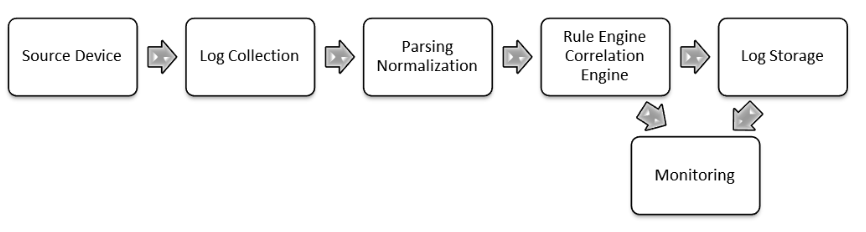
\includegraphics[width=0.8\textwidth]{assets/2_p2.png}
   \caption[Allgemeine Informationsfluss von \gls{SIEM}]
   {Allgemeine Informationsfluss eines \gls{SIEM} \\Quelle: \citep{Granadillo_SIEM} }
   \label{fig:SIEM_Allg_Informationsfluss}
   \centering
\end{figure}

In der Abbildung sehen wir, dass die Logdatei des \gls{Endpoint}s gesammelt werden und an dem Tool angepasst. Diese Information wird dann verarbeitet, um nach Muster zu suchen. Diese Daten werden schließlich gespeichern und zur Überwachung geschickt.

% Die folgende Abbildung zeigt eine allgemeine Architektur von Log-Analyse-Tools:

% \begin{figure}[H]
%    \centering
%    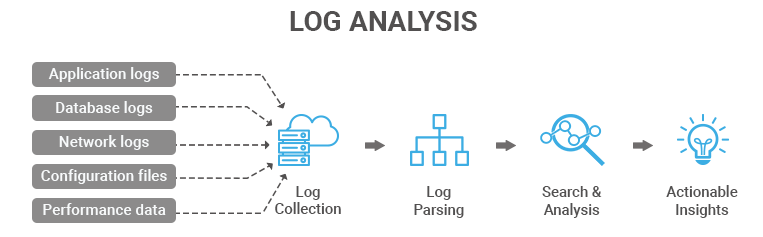
\includegraphics[width=0.8\textwidth]{assets/2.1_p2.png}
%    \caption[Allgemeine Struktur von Log-Analyse-Tools]
%    {Allgemeine Struktur von Log-Analyse-Tools\\Quelle: \citep{Tek-Tools_LGTArchitektur} }
%    \centering
% \end{figure}

% Den Informationsfluss eines Log Analyse Tools bildet folgende Grafik ab:

% \begin{figure}[H]
%    \centering
%    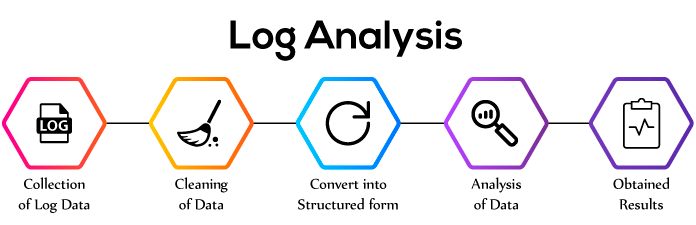
\includegraphics[width=0.55\textwidth]{assets/2.2_p2.png}
%    \caption[Allgemeine Informationsfluss von Log-Analyse-Tools]
%    {Allgemeine Informationsfluss von Log-Analyse-Tools\\Quelle: \citep{Neptune_LATInfoFluss} }
%    \centering
% \end{figure}

Aus bisheriger Abbildung stellen wir fest, dass \gls{SIEM} das Ergebnis der Integration von zwei wichtigen Komponenten ist, Datensammlung und Verarbeitung. Das Ziel dieser Software ist es die automatische Analyse zu ermöglichen, indem Daten kombiniert und bewertet werden können. In vielen Bereichen, wie Finanzen (\glsfirst{PCDISS}), Gesundheitswesen (\glsfirst{HIPAA}), sind \glsplural{SIEM} eine gesetzliche vorgegeben \citep{Jog_SIEM}. In Deutschland verpflichtet das \gls{IT-Sicherheitsgesetz 2.0} die Anwendungen solcher Lösungen, um Schädigung der \glsfirst{CIA} zu verhindern \citep{BSI_ITSG}. Log-Analyse-Tools sind seinerseits allgemeine Tools zu der Speicherung, Anpassung, Bewertung und Darstellung von Logdateien, ohne dass sie sich auf die Sicherheitsebenen fokussieren.


\subsection{Existierende SIEMs Lösungen und Log-Analyse-Tools}
% über Splunk schreiben, state of the art, nicht open source, aber andere müssen ähnliche funktionaliten haben
Die existierenden \glsplural{SIEM} und Log-Analyse-Tools werden in zwei Kategorien getrennt werden: \textit{\gls{Proprietary}} und  \textit{\gls{opensource}}. In folgenden Abschnitten präsentieren wir das proprietäre Tool Splunk, um einen Maßstab für unsere Auswahl zu definieren, wenn es um Funktionalität geht. Wir analysieren folgende Tools: %\glsplural{SIEM} und Log-Analyse-Tools: 

\begin{itemize}[noitemsep]
   \item Prelude %(nein)
   \item AlienVault \glsfirst{OSSIM} %(nein)
   \item FortiSIEM %(nein)
   \item Elastic Stack %(nein)
   \item Grafana integriert mit Loki %(ja)
\end{itemize}

%\textbf{\textcolor{red}{Wie konnte ich Grafana hier erwähnen? Grafane ist eher allgemein und nicht so zu Alert orientiert, habe ich hier gefunden: \href{https://www.metricfire.com/blog/grafana-vs-splunk/}{Splunk x Grafana} und hier \href{https://www.researchgate.net/publication/350730340_Implementation_of_Grafana_as_open_source_visualization_and_query_processing_platform_for_data_scientists_and_researchers}{What is Grafana}}  }

\subsubsection{Splunk}
Splunk, von dem gleichnamigen Unternehmen, wurde 2003 in den USA auf dem Markt gebracht \citep{Splunk_splunk}. Splunk ermögliche einfache Wartung, benutzerfreundliche \gls{GUI} und Skalierbarkeit \citep{Kazarov_Splunk}. Er gehört weltweit zu der meistverwendeten \gls{SIEM}-Lösung und zu ihren Kunden gehören große Konzerne wie Airbus, Coca-Cola, Intel und die Deutsche Bahn. Splunk bietet laut seiner Webseite folgende Funktionalitäten an \citep{Splunk_SPE}:

\begin{itemize}[noitemsep]
   \item Skalierbare Datenplattform 
   \item Risk-based Warnmeldung  
   \item Bedrohungserkennung mithilfe von \glsfirst{ML} 
   \item Automatische Aktualisierung von der Bedrohungs- und Schwachstelle-Database 
   \item Unkomplizierte Installation und Anwendung 
\end{itemize}

Die allgemeine Architektur und der Informationsfluss von Splunk unterscheidet sich nicht von der oben dargestellten Struktur in der Abbildung \ref{fig:SIEM_Allg_Struktur}, Seite \pageref{fig:SIEM_Allg_Struktur}, und Abbildung \ref{fig:SIEM_Allg_Informationsfluss}, Seite \pageref{fig:SIEM_Allg_Informationsfluss}. Da es sich hier um eine proprietäre Lösung handelt, lässt sich Splunk mit vielen anderen Funktionalitäten verwalten und erweitern. 

Die nächste Abbildung, \ref{fig:Allgemein_Splunk}, zeigt ein zusammenfassendes Diagramm über den Umfang des Informationsflusses von Splunk:

\begin{figure}[H]
   \centering
   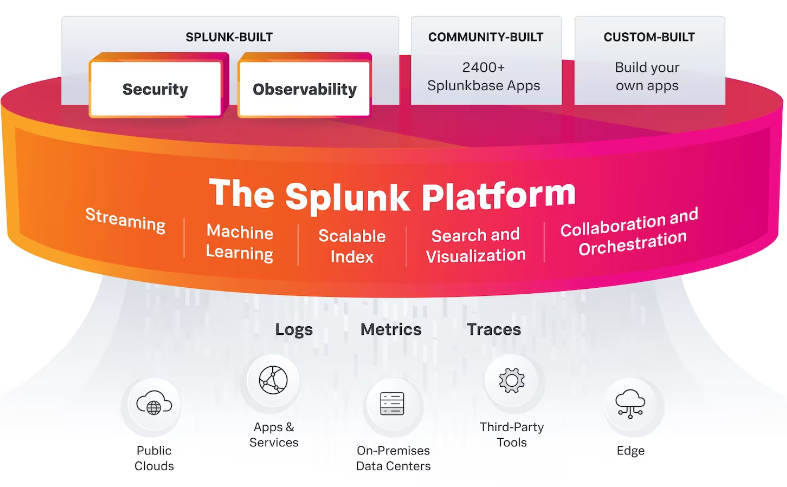
\includegraphics[width=0.7\textwidth]{assets/Splunk_informationsfluss.png}
   \caption[Allgemeine Informationsfluss von Splunk]
   {Allgemeine Informationsfluss von Splunk\\Quelle: \citep{Splunk_platform} }
   \label{fig:Allgemein_Splunk}
   \centering
\end{figure}

Auf dem Bild sehen wir unten die \glsplural{Endpoint}, dessen Daten und Logdateien von Splunk und seine \glsplural{plugin} und Funktionalitäten verarbeitet und analysiert werden.

Wie in anderen Tools, funktioniert die Bedrohungserkennung mithilfe von Regelsätzen, die aus \glsplural{usecases} können. Laut der Dokumentation existieren sie in folgenden Szenarien: Überwachung, Untersuchung und Erkennung. Die Software ist sowohl mit \gls{mitre} Matrix als auch mit \glsfirst{CKC} für die Gestaltung ihrer \glsplural{usecases} integriert \citep{Splunk_usecases}. 

In \citep{Su_SplunkDDOS} wurden Angriffe auf einem System simuliert und schließlich mit Splunk analysiert, um Gefahren zu identifizieren und diese im Voraus zu sehen. In \citep{Selvaganesh_SplunkBruteForce} wurde beschrieben, wie eine Splunk-Instanz installiert und konfiguriert wird, um spezifische \gls{bruteforce} zu erkennen.
 
\subsubsection{Prelude}
% suche nach Modulen, die man separat benutzen kann (Correlator)
Das im Jahr 2002 in Frankreich von Yoann Vandoorselaere released Tool Prelude zählt zu einer europäischen \gls{opensource} \gls{SIEM} Lösung. Laut dem Anbieter verfügt Prelude unter anderem folgende Funktionalitäten \citep{Prelude_SIEM}: 

\begin{itemize}[noitemsep]
   \item	Informationszentralisierung 
   \item	Datenaggregation und -Zusammenhang mit vordefinierten und von dem Nutzer angepassten Regeln 
   \item	Einbruchserkennungsmechanismen 
   \item	Datennormalisierung 
\end{itemize}

Die Anwendung besteht aus verschiedenen unabhängigen Modulen. Unter denen nennen wir Warnmeldung, Archivierung, Analyse und Verwaltung. Erstens gehört zu der zentralen Aufgabe dieser Lösung - es kan folgendens: Daten empfangen, normalisieren, Zusammenhänge erschließen und Meldungen generieren. Das zweite Modul \quotes{Archivierung} konzentriert sich auf die Speicherung und Verfügbarkeit der Daten. Der Analyse-Modul stett Daten in verschiedenen Formaten dar. Das letzte Modul dient dazu, die Anwendung zu steuern, Nutzer zu erstellen und deren Rechte zu konfigurieren \citep{EC_Prelude}. 

\newpage
Die folgende Abbildung,\ref{fig:Module_preludes}, zeigt die Integration verschiedener Module von Prelude und wie sie mit einander kommunizieren, um Analyse, Meldung und Speicherung zu generieren:

\begin{figure}[H]
   \centering
   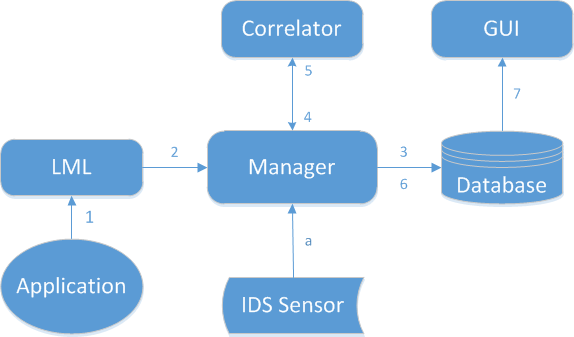
\includegraphics[width=0.5\textwidth]{assets/2_p3.png}
   \caption[Integration zwischen den Modulen von Prelude ]
   {Integration zwischen den Modulen von Prelude \\Quelle: \citep{Prelude_MU} }
   \label{fig:Module_preludes}
   \centering
\end{figure}

Aus der Abbildung und der Dokumentation können wir folgenden Informationsfluss erkennen - die Daten werden von Endanwendung generiert und zum Loganalyzer (Prelude \glsfirst{LML}) (1) geschickt, wo sie normalisiert und bewertet werden Für die Logs, wo es verdächtige Werte nach dem vordefinierten Regelsätze in \gls{LML} gibt, werden Warnmeldungen generiert. Diese Meldungen werden zum Manager Module (2) weitergeleitet. Der Correlator oben sucht nach einem Zusammenhang (5) zwischen anderen Daten. Das Ergebnis von Correlator wird wieder zum Manager (4) geschickt und danach zu der Datenbank (6). Schließlich stehen die Berichte in dem User-Interface zur Verfügung (7)\citep{Prelude_Doc}.

Die Architektur der Anwendung ermöglicht sowohl einen zentralisierten als auch einen dezentralisierten Aufbau. In der ersten funktioniert Prelude als zentral und empfängt Daten von verschiedenen Datenquelle und in den zweiten gibt es mehrere Instanzen von Preludes, dessen Ergenisse sich in einem \gls{GUI} darstellen lassen \citep{Prelude_MU}. 

\newpage
In der nächsten Abbildung, \ref{fig:Prelude}, sehen wir eine einfache Darstellung des Informationsflusses von Prelude:

\begin{figure}[H]
   \centering
   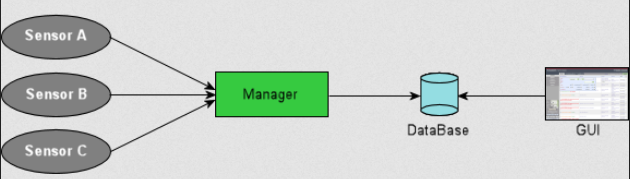
\includegraphics[width=0.7\textwidth]{assets/2_p4.png}
   \caption[Informationsfluss in Prelude]
   {Informationsflussin Prelude \\Quelle: \citep{Prelude_MU} }
   \label{fig:Prelude}
   \centering
\end{figure}

Die dezentralisierte Umgebung von Preludes lässt sich in der folgenden Abbildung darstellen:

\begin{figure}[H]
   \centering
   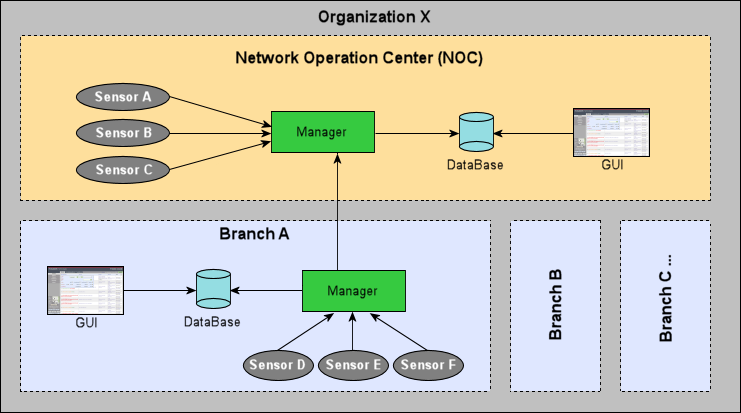
\includegraphics[width=0.8\textwidth]{assets/2_p5.png}
   \caption[Erweiterte Architektur von Prelude mit dezentralisierten Datenquellen und Datenverarbeitung]
   {Erweiterte Architektur von Prelude mit dezentralisierten Datenquellen Datenverarbeitung\\Quelle: \citep{Prelude_MU} }
   \centering
\end{figure}

\newpage
%Die Publikationen über Preludes fokussieren sich auf die Entwicklung, Implementation und unternehmerische Anwendung dieses Tools. 
In \citep{Grammatikis_Prelude} wurde Preludes, AlienVault und Cyberoam iView anhand technischer und nutzerfreundlicher Kriterien zu verglichen. Von diesn Kriterien nennen wir folgende \citep{Grammatikis_Prelude}: 

\begin{itemize}[noitemsep]
   \item \textbf{technische Kriterien}
   \begin{itemize}[noitemsep]
      \item Echtzeige Leistung\textit{Real-time performance}, 
      \item Umfang und Flexibilität der Meldungen \textit{Range and flexibility of reporting}
      \item Zusammenhang von Warnmeldung \textit{Alert correlation}
   \end{itemize}

   \item \textbf{nutzerfreundliche Kriterien}
   \begin{itemize}[noitemsep]
      \item Vollständige Dokumentation \textit{Documentation comprehensiveness}
      \item Komplexität der Installation \textit{Complexity of the installation process}
      \item Komplexität der Einstellung \textit{Complexity of the system configuration}
   \end{itemize}
\end{itemize}

In den technischen Kriterien lag Prelude auf dem dritten Platz und bei Benutzerfreundlichkeit bekam Prelude den ersten. 

%Auch in den nicht wissenschaftlichen Publikationen existiert eine begrenzte Anzahl von Texten über Preludes. Die existierenden Texte kommentieren ganz zusammenfassend die ausreichende Dokumentation und heben hervor, dass es eher eine in Europa verbreitete Lösung ist.

\subsubsection{AlienVault OSSIM}
AlienVault OSSIM ist eine im Jahr 2007 entwickelte \gls{opensource} \gls{SIEM} Lösung. Im Jahr 2018 wurden sie von der Firma AT\&T Communication gekauft  \citep{CBN_AV}. In der Beschreibung des Anbieters steht, dass er sie auch dabei unterstützt, Daten zu sammeln, zu normalisieren und zu bewerten. Er behauptet auch, dass sein Tool in der Lage ist, Schwachstellen und Angriffe zu erkennen, das Verhältnis zu beobachten und Datenzusammenhänge zu erschließen \citep{ATT_AVO}. 

AlienVault hat eine kostenpflichtige Version, die Alien Vault \glsfirst{USM} heißt. Auf der Webseite von AT\&T steht, dass es keine dedizierte Dokumentation für die \gls{opensource} Version AlienVault OSSIM gibt, da viele Funktionalitäten von der kostenpflichtigen Version stammen \citep{ATT_AVO}. 

\newpage
Die folgende Abbildung, \ref{fig:AlienVault_Architektur}, zeigt das von dem Anbieter freigelegte Architekturdiagramm von der \gls{USM} Version:

\begin{figure}[H]
   \centering
   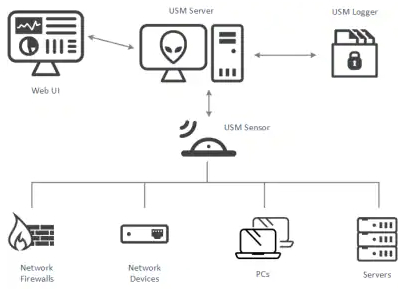
\includegraphics[width=0.6\textwidth]{assets/2_p6.png}
   \caption[Architekturdiagramm von AlienVault \gls{USM}]
   {Architekturdiagramm von AlienVault \gls{USM} \\Quelle: \citep{ATT_AVO} }
   \label{fig:AlienVault_Architektur}
   \centering
\end{figure}

Unten im Bild sehen wir die mit einem Sensor verbundenen \glsplural{Endpoint}. Der Sensor analysiert die Daten und leitet diese zu dem Server weiter \citep{AV_Sensor}. Die Daten werden auf Logger (rechts) gespeichert und über die \gls{GUI} (links) dargestellt. 

Laut der Website Comparitech steht AlienVault auf dem 13ten Platz von den bestbewertetsten \gls{SIEM}-Lösungen. Die Seite beschreibt auch, dass zu dem Tool einen \gls{IDS}, ein Verhaltensüberwachungssystem und einen Schwachstellen-Scanner integriert sind. Die Anwendung ist auch mit der Plattform \gls{OTX} verbunden - diese ermöglicht eine Teilung von Informationen über die Schwachstelle. Comparitech highlighted, dass die Anwendung wegen ihrer niedrigen Kosten besser für kleine oder mittelständige Unternehmen geeignet ist \citep{comparitech_SIEM}. 

Die Anwendung bietet konsistenten Daten Zusammenhang an und soll das Auftauchen von \gls{falsch positiv} vermeiden. AlienVault kommt mit vordefinierten \glsplural{usecases}, die dabei unterstützen, gewöhnliche Angriffsszenarien zu erkennen. Die Installation, die Einstellung und die Integration mit anderen Tools ist auch benutzerfreundlich \citep{Gomes_AV}. \citep{Nabil_AV} behauptet, dass für viele Quellen eine manuelle Normalisierung der Logdatein notwendig ist.

%Die Anwendung hat aber einen zuverlässigen Berichtsmechanismus. 

%Während unserer Recherche gab es wenig wissenschaftliche Literatur, die sich um AlienVault OSSIM kümmert.
Die meisten Publikationen über AlienVault OSSIM stammen aus kommerziellen Quellen und diese konzentrierten sich auf eine kostenpflichtige \gls{SIEM}-Lösung von AT\&T.

\subsubsection{FortiSIEM}
FortiSIEM ist eine \gls{SIEM}-Lösung von der US-amerikanische Firma Fortinet. Fortinet kaufte im Jahr 2016 das Unternehmen AccelOps und dessen \gls{SIEM}-Lösung und benannte es zum FortSIEM \citep{Fortinet_Press}. 

Laut dem Anbieter hat FortiSIEM eine robuste Integration mit anderen Tools und lässt sich leicht und einwandfrei skalieren. Andere Versionen des Tools sind mit \glsfirst{ML} integriert, sodass die Anwendung auch Verhältnisanalysen durchführen kann \citep{Fortinet_Solutions}. Das Tool bietet auch eine umfangreiche und ausführliche Dokumentation an. 

Die nächste Abbildung, \ref{fig:FortiSIEM}, zeigt die skalierbare Architektur von FortiSIEM:

\begin{figure}[H]
   \centering
   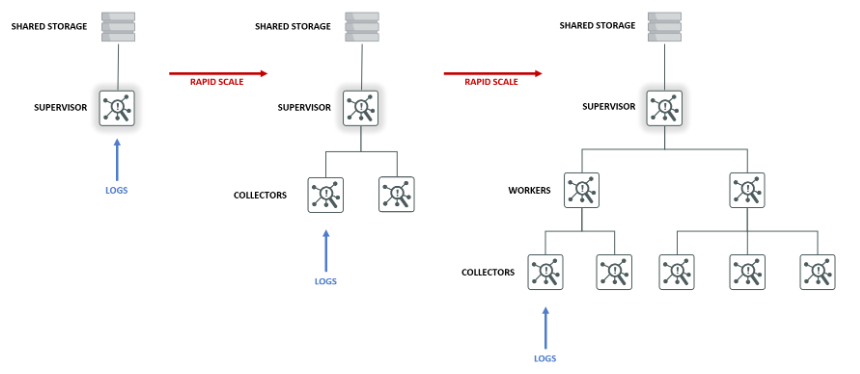
\includegraphics[width=1\textwidth]{assets/2_p7.png}
   \caption[Skalierbare Architektur von FortiSIEM]
   {Skalierbare Architektur von FortiSIEM \\Quelle: \citep{Fortinet_Arch} }
   \label{fig:FortiSIEM}
   \centering
\end{figure}


%Auch zu dieser \gls{SIEM}-Lösung ist die wissenschaftliche Produktion eingeschränkt.
\newpage 
\citep{Ramires_fortisiem} behauptet, dass FortiSIEM eine schnelle Erkennung von Angriffen bietet und über \glsfirst{NOC} Funktionalität verfügt, wie Netzmanagement. 

Wie andere \glspl{SIEM} Lösungen, hat FortiSIEM folgende Funktionalitäten:

\begin{itemize}[noitemsep]
   \item Datensammlung und Normalisierung
   \item Daten Zusammenhang
   \item Generierung von Berichten
   \item Warnmeldungen
   \item Datenauswertung
\end{itemize}

\subsubsection{Elastic Stack}
Elastic Stack stammt aus der Verbindung von drei Tools: Elasticsearch, Logstash und Kibana. Erstes ist eine Such-und Analyse-Maschine. Das Zweite ist eine serverseitige Anwendung zur Datenverarbeitung, -Weiterleitung und Sammlung von Logdateien. Schließlich Kibana \label{kibana} ist eine \gls{abfragesprache} dafür zuständig, Daten zu filtern und visuelle Darstellungen in einem Grafik-Format auszugeben \citep{packt_elkstack}. Von diesen drei Tools Logstasch ist das einzige \gls{opensource} \citep{elastic_OSI}. Obwohl die anderen zwei 
kostenlos verwendet werden können, gehören sie nicht zu der \gls{opensource} Kategorie \citep{OpenSource_Def}. Dieses Tool besitzt viele Eigenschaften einer \gls{SIEM}-Lösung und wird von vielen SOC verwendet, ist aber für viele Experten, kein \gls{SIEM} für sich, da es über keine Warnmeldungssystem, Daten Zusammenhang und Vorfälleverwaltung verfügt \citep{Miller_ELK}. Diese und anderen Funktionalitäten lassen sich aber durch \glsplural{plugin} integrieren. 

\newpage
Die nächste Abbildung, \ref{fig:Intregation_ELK}, stellt die Architektur von Elastic Stack mit ihren integrierten Elementen dar:

\begin{figure}[H]
   \centering
   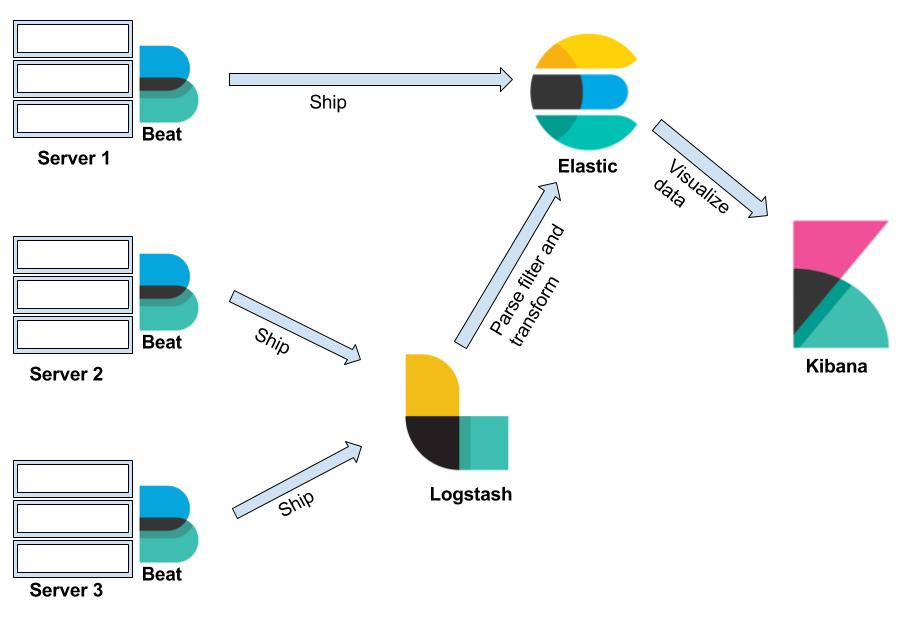
\includegraphics[width=0.8\textwidth]{assets/2_p8.png}
   \caption[Integration zwischen Elasticsearch, Logstash und Kibana]
   {Integration zwischen Elasticsearch, Logstash und Kibana\\Quelle: \citep{packt_elkstack} }
   \label{fig:Intregation_ELK}
   \centering
\end{figure}

Die Beats auf dem Bild sind an der \glsplural{Endpoint} installiert und leiten Daten entweder zu Elasticsearch oder zu Logstash weiter, wo sie schließlich bearbeitet werden \citep{Jain_LMELK}. 

In \citep{Advani_elkstakc} wird über die Log Analyse-Funktionalitäten von Elastic Stack und die Unterstützung bei Normalisierung und Indexierung von Daten für eine lesbare Ausgabe recherchiert. Die Skalierbarkeit wurde in der Studie von \citep{Wang_elkwifi} erwähnt, wo Elastic Stack für Wi-Fi Logging eingesetzt wurde. 

Die offizielle Dokumentation von Elastic Stack beschreibt, dass die Anwendung folgende Funktionalitäten besitzt \citep{elastic_docs}: 

\begin{itemize}[noitemsep]
   \item Datensuche, -Normalisierung, -Analyse und 
   \item Speicherung
   \item visuelle Ausgabe
\end{itemize}

Die folgende Abbildung, \ref{fig:ElasticKomponenten}, aus der offiziellen Dokumentation, zeigt die Aufteilung der Funktionalitäten pro Element von Elastic Stack:

\begin{figure}[H]
   \centering
   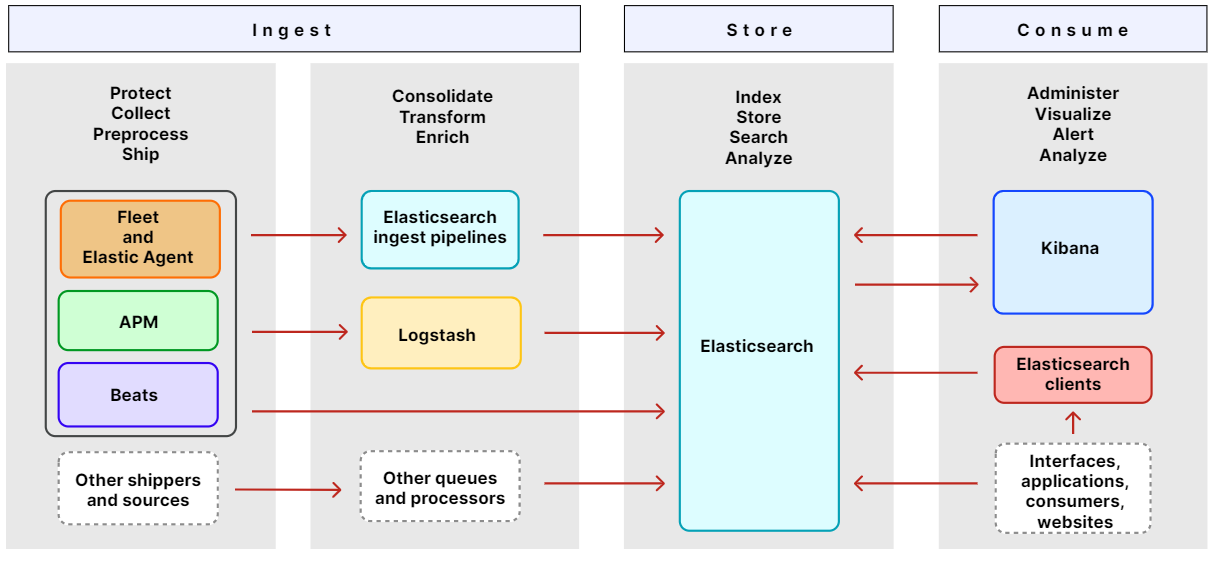
\includegraphics[width=0.8\textwidth]{assets/2_p9.png}
   \caption[Aufteilung der Funktionalitäten zwischen den Komponenten]
   {Aufteilung der Funktionalitäten zwischen den Komponenten\\Quelle: \citep{elastic_docs}}
   \label{fig:ElasticKomponenten}
   \centering
\end{figure}

Die wissenschaftliche Publikation über Elastic Stack ist vielfältiger als bei anderen recherchierten Tools. Die Mehrheit von denen sich eher mit dem Logging als mit den \gls{SIEM}-Eigenschaften der Anwendung beschäftigt.

\subsubsection{Grafana}
Von allen recherchierten Lösungen ist Grafana die Einzige, die weder \gls{SIEM} noch Log-Analyse-Tools ist. Grafana wird als Plattform für Visualisierung von Daten beschrieben. Mit dem Tool ist es möglich eine Graphik zu erstellen und Meldungen zu generieren. Das Ziel der Anwendung ist, Information in einer einfachen und verständlichen Art und Weise zur Verfügung zu stellen \citep{redhat_grafana}.  

Im Jahr 2014 wurde Grafana von der Firma Grafana Labs veröffentlicht. Das Tool basiert auf Kibana3,\ref{kibana}. Ursprünglich sollte Grafana ein einfacheres Bearbeitungstool für Grafiken sein und ermöglichen, Datenanfragen unkomplizierter zu machen. Die neuste Version, 9.4.3. wurde im März 2023 veröffentlicht und bietet viele Funktionalitäten an. Es ist auch möglich das Tool mithilfe von  \glsplural{plugin} zu erweitern \citep{Oedegaard_historyGrafana}.. 

In der Webseite betont der Anbieter, dass Grafana die Zentralisierung und Zugang von Daten vereinfachen. Alle Art von Daten lassen sich analysieren und darstellen, von der Leistung von Anwendungen bis Verkaufsdaten und Krankheitsfällen. Die Anwendung soll auch den Zusammenhang von Daten ermöglichen, um wichtige Informationen herauszunehmen \citep{Grafana_Grafana}.

Grafana ist auch mit dem Logging Tool Loki und Promptail integriert. Promtail ist für Sammlungen der Logdateien und Weiterleitung an Loki zuständig. Promptail wird an jeden \gls{Endpoint} installiert. Die Logdatein werden als Stream zu Loki geschickt und diese Streams werden dann identifiziert mithilfe von Index. Jeder Stream bezieht sich auf eine Gruppe von Logdateien. Der Inhalt der Logdateien bleiben aber ohne Index \citep{Grafana_fundamentals}. Promtail ist so konzipiert, um Logdateien nur zur Grafana Loki oder zu einem anderen Promtail zu schicken. Er kann nach Logdatei entdecken und dekomprimieren \citep{Grafana_Promtail}. Diese Daten können dann in Grafana mithilfe der \gls{abfragesprache} LogQL aufgerufen werden. Schließlich können Warnmeldungen mit spezifischen Regelsätze in \gls{logql} generiert werden, die in dem Alerting Tool von Grafana eingeführt werden \citep{Grafana_loki}. Auf der nächsten Abbildung, \ref{fig:Integration_Loki_Promtail_Grafana}, wird die Struktur von Grafana Loki  dargestellt:

\begin{figure}[H]
   \centering
   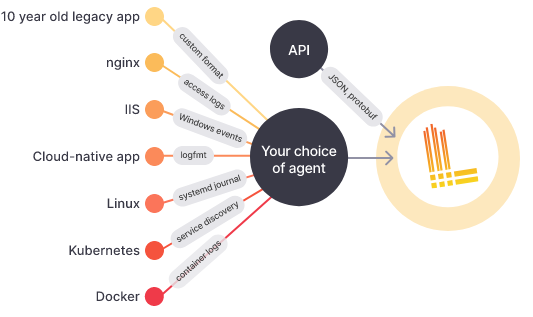
\includegraphics[width=0.8\textwidth]{assets/2_p10.png}
   \caption[Integration von Log-Quellen mit Promptail, Loki und Grafana]
   {Integration von Log-Quellen mit Promptail (links), Loki (mitte) und Grafana (rechts) \\Quelle: \citep{Grafana_Logs}}
   \label{fig:Integration_Loki_Promtail_Grafana}
   \centering
\end{figure}

Das Tool hat eine umfangreiche Dokumentation, die ausführlich erklärt, wie es zu installieren, bedienen und mit anderen Tools integrierbar ist. 

%\newpage
%Obwohl Grafana nicht spezifisch für den Sicherheitsbereich konzipiert wurde, kann das Tool so eingerichtet werden, dass spezifische Logdateien gesammelt, bearbeitet und analysiert werden. Die Warnmeldung lässt sich mit Regeln oder Filter definieren. In einer Recherche von 2022 wurde Grafana dafür benutzt, Daten aus Netzwerkverkehr graphisch darzustellen \citep{Manases_grafananetwork}. 

Die wissenschaftlichen Literatur über Grafana konzentriert sich eher auf die Anwendung des Tools für die grafische Darstellung von Daten als für ihre Nutzung in dem Sicherheitsbereich. Eine Recherche, z.B., wollte das Ergebnis von der Überwachung von Cloud-basierten Systemen, von Netzwerkaktivitäten und von Netzwerkverkehr mithilfe von Grafana darstellen \citep{Manases_grafananetwork}. 
Die wissenschaftliche Recherche über die Implementierung und Integration von Grafana mit anderen Tools zum Sicherheitszweck ist neu und bietet deshalb viele  Perspektive für das Weiterlernen an.

\subsection{Auswahlkriterium}
Der Erwerb einer \gls{SIEM} Lösung würde wahrscheinlich die Anforderungen dieser wissenschaftlichen Arbeit decken. Da solche Lösungen meistens (oder alle) \gls{Proprietary} und kostenpflichtig sind, legten wir als Auswahlkriterium fest, dass die Anwendungen für unsere Arbeit \gls{opensource} sein müssen. Deshalb arbeiten wir mit Grafana, Loki und Promtail.

In den nächsten Kapiteln beschäftigen wir mit der Integration dieser Tools, um eine ähnliche \gls{SIEM} Lösung zu präsentieren. Wir beschreiben die Installation, Einstellungen und Sammlungen von Logdateien und nachdem die Grundfunktionalitäten eingerichtet sind und einwandfrei funktionieren, untersuchen wir anhand der \glsfirst{ttp} der \gls{mitre} Matrix Regelsätze für die Erkennung und Warnmeldung von potenziellen Angriff. Unser Ziel ist Grafana, Loki und Promtail so einzustellen, dass es in der Lage ist, die Muster dieser Angriffe zu erkennen und darüber zu berichten.
